\section{ApproxPilot-SE Methodology}
\label{sec:method}

ApproxPilot-SE targets system-level design space exploration for approximate accelerators with multiple configurable arithmetic sites. Given a target RTL design and a pre-characterized approximate arithmetic-unit library, the framework constructs a legal configuration space, represents each candidate over the shared RTL topology, and estimates its hardware cost and application quality using learned PPA and QoR surrogates. The overall framework is illustrated in Fig.~\ref{fig:framework}.

A central feature of ApproxPilot-SE is that surrogate learning and design space exploration are coupled rather than treated as two isolated stages. The current surrogates guide the search toward competitive regions of the design space, while Pareto-relevant candidates are selected for ground-truth logic synthesis and application-level evaluation. Their measured PPA and QoR values are then incorporated into the training set to update the surrogates before the next search round. In this way, the search determines where new measurements are collected, and the resulting measurements reshape the models that drive subsequent exploration. After the iterative process, the updated surrogates support a larger final search, whose selected candidates are evaluated using ground-truth system-level measurements to construct the reported Pareto front.

\begin{figure*}[t]
    \centering
    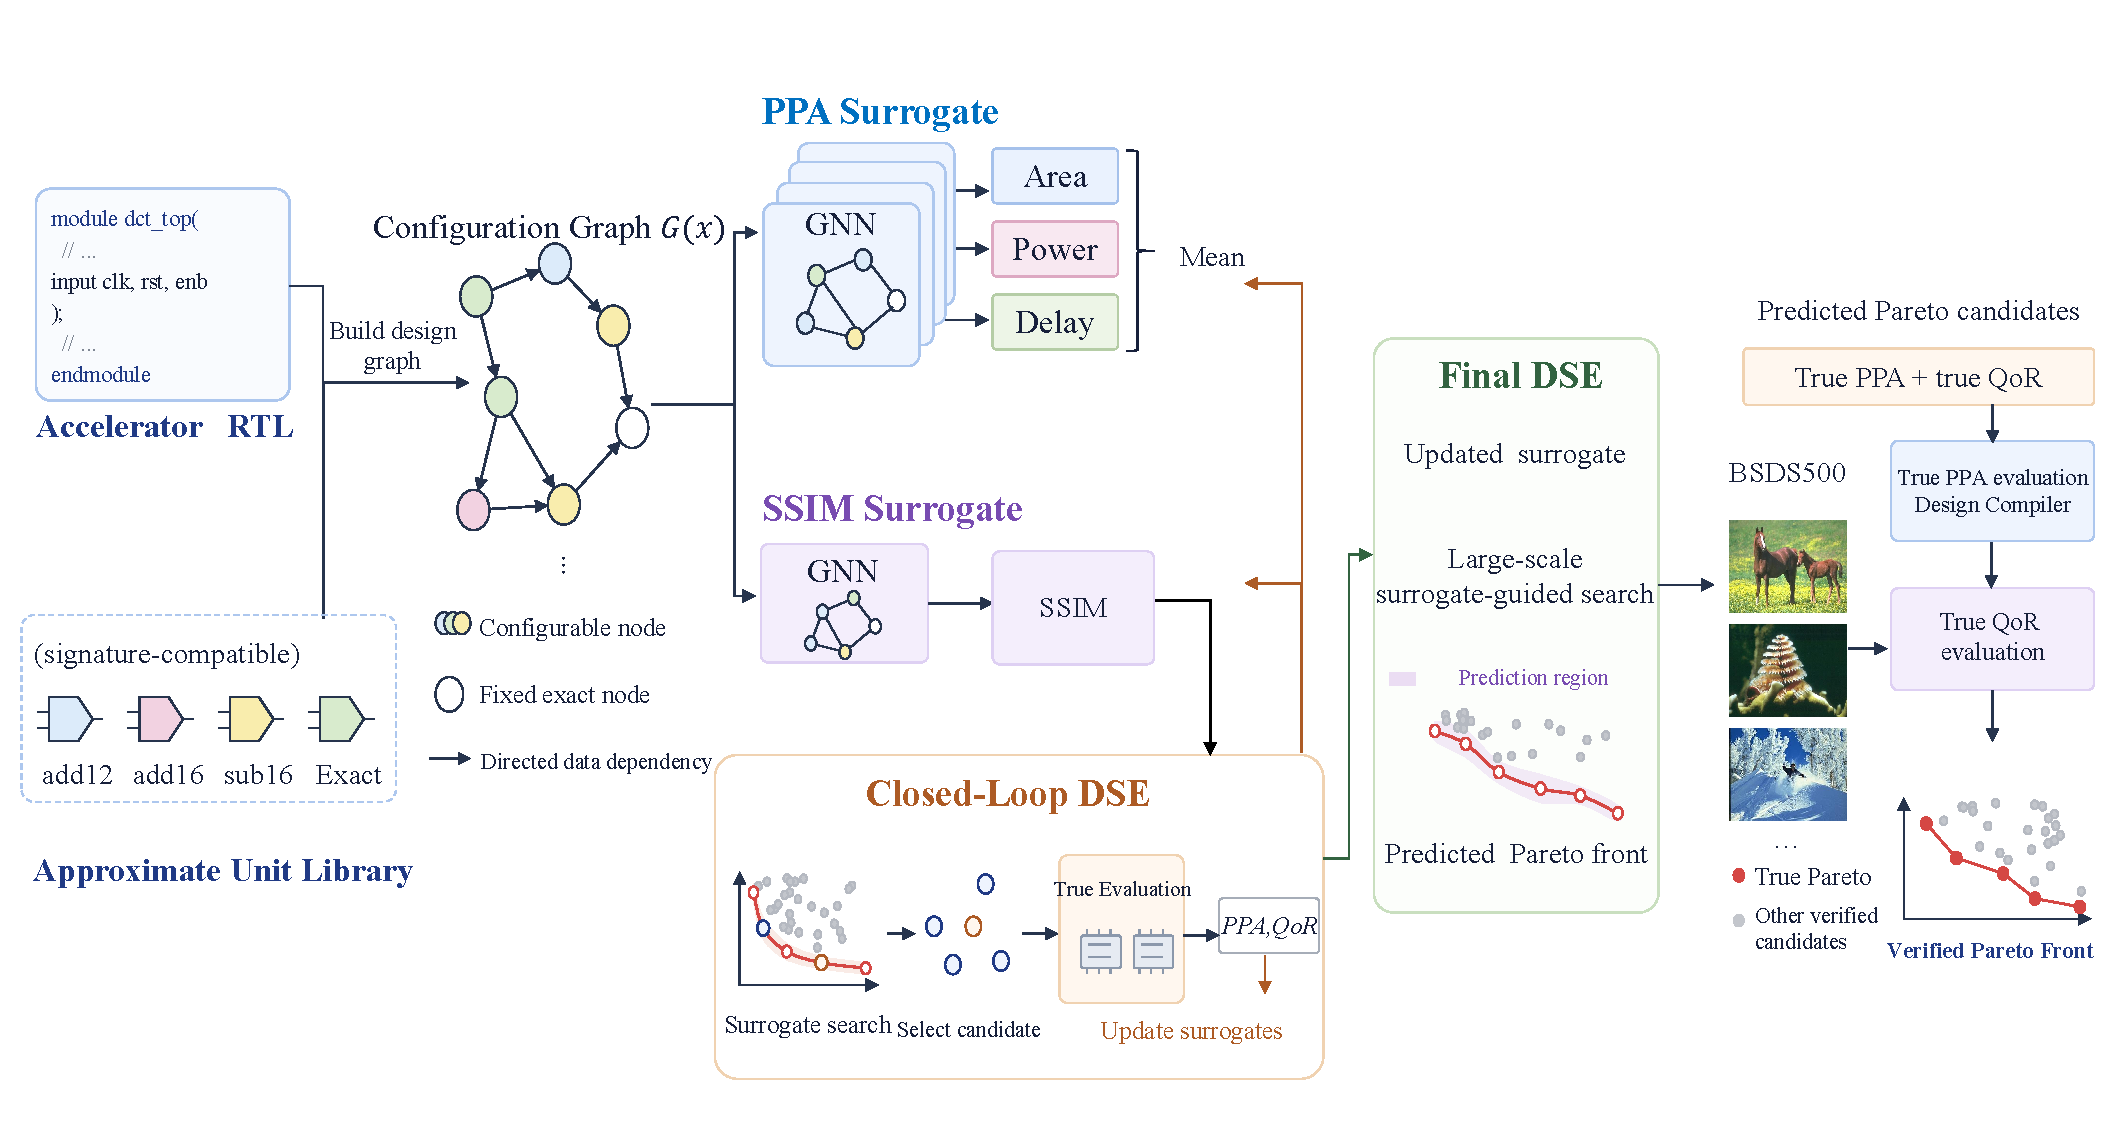
\includegraphics[width=0.98\textwidth]{figures/framework_v4.pdf}
    \caption{Overview of ApproxPilot-SE. Candidate accelerator configurations are represented on the RTL graph and evaluated by PPA and QoR surrogates. Pareto-relevant candidates identified during DSE receive ground-truth PPA and QoR evaluations, and the resulting labels are used to update the surrogate models for subsequent search rounds. The final Pareto front is reconstructed exclusively from ground-truth system-level evaluations.}
    \label{fig:framework}
\end{figure*}

ApproxPilot-SE consists of three closely connected components: configuration-aware graph modeling, system-level PPA and QoR surrogate prediction, and co-evolving surrogate-assisted DSE. The following subsections describe these components, with particular emphasis on the timing-domain path aggregation used for Delay modeling and the iterative interaction between surrogate learning and search.


\subsection{Configuration Space and Graph Representation}
\label{sec:configuration_graph}

The design space of ApproxPilot-SE is defined directly over the legal implementations of the configurable arithmetic sites in the target RTL. This formulation provides a unified representation for Exact and Approximate implementations while preserving the structural context in which each implementation operates.

Let
\begin{equation}
    \mathcal{V}_{\mathrm{cfg}}=\{1,2,\ldots,N\}
\end{equation}
denote the set of configurable arithmetic sites in the target accelerator. For site $i$, let $e_i$ denote its exact implementation and $\mathcal{A}_i$ the set of approximate arithmetic units compatible with its RTL interface. The legal implementation set of site $i$ is therefore defined as
\begin{equation}
    \mathcal{C}_i=\{e_i\}\cup\mathcal{A}_i .
    \label{eq:site_state}
\end{equation}
A complete accelerator configuration is represented by
\begin{equation}
    \mathbf{x}=[x_1,x_2,\ldots,x_N],
    \qquad
    x_i\in\mathcal{C}_i .
    \label{eq:configuration}
\end{equation}

This formulation places Exact and Approximate implementations in the same discrete configuration space. Selecting $e_i$ keeps site $i$ exact, whereas selecting an element of $\mathcal{A}_i$ assigns the corresponding approximate arithmetic unit. The candidate set may differ across sites because legality is determined by the operation type, signedness, and input/output interfaces of the original RTL operator. Arithmetic nodes that are structurally fixed to Exact implementations are excluded from the design variables but remain in the complete RTL graph, thereby preserving the original data dependencies.

For a configuration $\mathbf{x}$, its ground-truth system response is defined as
\begin{equation}
    \mathbf{y}(\mathbf{x})
    =
    \left[
    A(\mathbf{x}),
    P(\mathbf{x}),
    D(\mathbf{x}),
    Q(\mathbf{x})
    \right],
    \label{eq:system_response}
\end{equation}
where $A(\mathbf{x})$, $P(\mathbf{x})$, and $D(\mathbf{x})$ denote post-synthesis Area, Power, and Delay, respectively, and $Q(\mathbf{x})$ denotes application-level quality of result (QoR). Using the fully exact accelerator as the hardware reference, the multi-objective search operates on
\begin{equation}
    \mathbf{f}(\mathbf{x})
    =
    \left[
    \frac{A(\mathbf{x})}{A_{\mathrm{ex}}},
    \frac{P(\mathbf{x})}{P_{\mathrm{ex}}},
    \frac{D(\mathbf{x})}{D_{\mathrm{ex}}},
    1-Q(\mathbf{x})
    \right].
    \label{eq:objectives}
\end{equation}
The optimization therefore seeks nondominated accelerator configurations that balance application quality against system-level hardware cost, rather than optimizing the local characteristics of individual approximate units in isolation.

To model the system-level behavior induced by different configurations, ApproxPilot-SE represents the target accelerator as a directed graph
\begin{equation}
    G(\mathbf{x})=(V,E,\mathbf{X}(\mathbf{x})),
    \label{eq:graph}
\end{equation}
where $V$ contains arithmetic-operation nodes, $E$ captures directed RTL data dependencies, and $\mathbf{X}(\mathbf{x})$ denotes configuration-dependent node attributes. Candidate configurations of the same accelerator share the underlying RTL topology, while the implementation assigned to each configurable node and its associated attributes vary with $\mathbf{x}$. This representation allows the surrogate models to distinguish different Exact/Approximate assignments while retaining the structural context in which those assignments affect the complete accelerator.

Each node representation combines two complementary types of information. The first characterizes the RTL operator and its structural context, including operation and interface attributes as well as its position in the directed dataflow graph. The second characterizes the implementation selected by the current configuration, including unit-level hardware properties and numerical-error descriptors. These local descriptors capture the behavior of individual arithmetic implementations, whereas their system-level effects are learned over the complete RTL graph rather than approximated by directly accumulating unit-level metrics.

The resulting configuration-aware graph provides a common structural basis for the PPA and QoR surrogates. The PPA branch learns how local implementation choices interact through the RTL topology to determine Area, Power, and Delay, whereas the QoR branch additionally exploits approximation-error characteristics to capture their impact on application-level quality. The two surrogate models are described next.





% B PPA 与 QoR 代理模型
\subsection{PPA and QoR Surrogate Models}
\label{sec:surrogate_models}

ApproxPilot-SE employs separate PPA and QoR surrogates to rapidly evaluate the hardware cost and application quality of candidate configurations. For a given accelerator, the RTL data-dependency topology remains fixed, while the attributes of configurable nodes change with the selected Exact or Approximate implementations. The surrogates therefore learn how different arithmetic-unit assignments translate into system-level behavior over the same underlying computation graph.

The PPA surrogate uses a four-layer directed graph encoder with 128-dimensional hidden representations. Each node is initialized from its RTL attributes, structural information, and the characteristics of the currently selected arithmetic implementation. Information is then propagated along directed RTL dependencies so that the resulting node representation captures both the local implementation and its upstream computation context.

Area and Power are predicted using two independent learned graph readouts. Each readout assigns objective-specific importance to the encoded nodes, forming a graph-level representation tailored to the corresponding hardware metric. This representation is combined with configuration-level global features and passed to an independent regression head to estimate post-synthesis Area or Power. Unit-level physical characteristics describe the local implementations, while their system-level effects are learned from the complete accelerator graph rather than obtained by directly accumulating individual unit costs.

Delay shares the same directed graph encoder but uses a different readout. Because system delay is strongly shaped by directed data paths and competition among them, ApproxPilot-SE preserves path structure when constructing the Delay representation instead of relying on conventional global aggregation. The resulting timing-domain path aggregation is described in Section~\ref{sec:path_aggregation}.

The QoR surrogate is implemented as a separate five-layer GraphSAGE model with 128-dimensional hidden representations. In addition to RTL and configuration information, its node features include numerical-error descriptors of the selected arithmetic units. The encoded node representations are jointly used to predict the quality response for multiple application inputs, whose mean serves as the configuration-level QoR used during DSE. This model directly captures the mapping from arithmetic-unit assignments to application-level output quality over the complete computation graph.

PPA and QoR prediction use ensembles of five and three independently trained models, respectively, with the ensemble mean serving as the surrogate estimate during search. For a candidate configuration $\mathbf{x}$, the two branches jointly provide
\begin{equation}
    \left[
    \hat{A}(\mathbf{x}),
    \hat{P}(\mathbf{x}),
    \hat{D}(\mathbf{x}),
    \hat{Q}(\mathbf{x})
    \right],
\end{equation}
enabling efficient system-level evaluation of a large number of candidate designs during multi-objective DSE.






% C 时序域路径聚合

\subsection{Timing-Domain Path Aggregation}
\label{sec:path_aggregation}

System Delay is governed by the propagation of signals along directed computation paths. The timing impact of an arithmetic implementation therefore depends on both its local characteristics and its position within the RTL dataflow. ApproxPilot-SE incorporates this path dependency through a timing-domain readout built on the node representations produced by the directed graph encoder.

Let $\mathbf{h}_v$ denote the encoded representation of node $v$. Within each timing domain, node states are propagated in topological order so that information accumulated along upstream paths is retained. For node $v$ in timing domain $d$, let $\mathrm{Pred}_d(v)$ denote its in-domain predecessors. The path state is defined as

\begin{equation}
    \mathbf{z}_{d,v}
    =
    \mathbf{h}_v
    +
    \max_{u\in\mathrm{Pred}_d(v)}
    \mathbf{z}_{d,u},
    \label{eq:path_recurrence}
\end{equation}

where the maximum is taken element-wise over the feature dimensions. For a source node within the timing domain,

\begin{equation}
    \mathbf{z}_{d,v}=\mathbf{h}_v .
    \label{eq:path_source}
\end{equation}

This recurrence accumulates node information along directed paths while retaining the strongest responses when multiple predecessor paths converge. Processing nodes in topological order allows each path state to summarize the implementation and structural information propagated from its upstream computation.

The resulting states are aggregated within each timing domain and then across timing domains:

\begin{equation}
    \mathbf{r}_D
    =
    \max_d
    \left(
        \max_{v\in V_d}
        \mathbf{z}_{d,v}
    \right),
    \label{eq:delay_readout}
\end{equation}

where $V_d$ denotes the nodes belonging to timing domain $d$. The resulting representation is combined with the configuration-level global features and mapped to the system-level Delay prediction:

\begin{equation}
    \hat{D}(\mathbf{x})
    =
    f_D
    \left(
        [\mathbf{r}_D \Vert \mathbf{g}(\mathbf{x})]
    \right).
    \label{eq:delay_prediction}
\end{equation}

The path recurrence operates on GNN-encoded node representations, while the final mapping to Delay is learned directly from system-level Delay labels. Consequently, the model incorporates RTL path order and path competition without requiring explicit critical-path node labels. The resulting path-aware representation provides the Delay surrogate used by ApproxPilot-SE during design space exploration.









% D 代理模型与 DSE 的协同演化
\subsection{Co-Evolving Surrogates and DSE}
\label{sec:coevolving_dse}

ApproxPilot-SE couples surrogate learning with multi-objective DSE through iterative ground-truth feedback. Let $\mathcal{D}_r$ denote the labeled set available at the beginning of round $r$. The PPA and QoR surrogates are trained on $\mathcal{D}_r$ and used to evaluate a large number of candidate configurations during search. Pareto-relevant candidates identified by the current search are then evaluated at the system level, and the resulting measurements are incorporated into the labeled set before the next round.

At round $r$, the current surrogates provide
\begin{equation}
    \left[
    \hat{A}_r(\mathbf{x}),
    \hat{P}_r(\mathbf{x}),
    \hat{D}_r(\mathbf{x}),
    \hat{Q}_r(\mathbf{x})
    \right]
\end{equation}
for each candidate configuration $\mathbf{x}$. ApproxPilot-SE uses these predictions to drive an NSGA-III search~\cite{deb2014nsga3} over the legal configuration space. Previously evaluated configurations are excluded from acquisition, and the remaining candidates are ranked by predicted nondominated fronts over the four objectives. Candidates are selected front by front so that ground-truth evaluations are concentrated on configurations with high optimization relevance.

When the remaining acquisition budget cannot accommodate an entire front, crowding distance~\cite{deb2002nsga2} is used to select candidates from that front. A larger crowding distance indicates a sparser neighborhood in the objective space; prioritizing such candidates preserves diverse PPA--QoR tradeoffs within the same nondomination level. The selected batch at round $r$ is denoted by $\mathcal{B}_r$.

Each configuration in $\mathcal{B}_r$ is then evaluated using logic synthesis and application-level execution to obtain
\begin{equation}
    \mathbf{y}(\mathbf{x})
    =
    \left[
    A(\mathbf{x}),
    P(\mathbf{x}),
    D(\mathbf{x}),
    Q(\mathbf{x})
    \right],
    \qquad
    \mathbf{x}\in\mathcal{B}_r .
\end{equation}
The newly measured configurations are added to the labeled set as
\begin{equation}
    \mathcal{D}_{r+1}
    =
    \mathcal{D}_{r}
    \cup
    \left\{
    (\mathbf{x},\mathbf{y}(\mathbf{x}))
    \mid
    \mathbf{x}\in\mathcal{B}_r
    \right\}.
    \label{eq:data_update}
\end{equation}

Both the PPA and QoR surrogates are retrained on $\mathcal{D}_{r+1}$ and immediately used in the next round of DSE. The search therefore determines where new ground-truth measurements are collected, while the newly acquired measurements reshape the surrogates that guide subsequent exploration. This bidirectional interaction constitutes the co-evolution of surrogate models and DSE in ApproxPilot-SE.

After the feedback rounds, the updated surrogates are used for a larger final search. A final set of Pareto-relevant candidates is selected from the predicted archive and evaluated using the same ground-truth PPA and QoR flow. The reported Pareto front is then reconstructed from the measured final candidates together with the Exact reference design. Surrogates determine where the design space is explored, whereas the reported hardware tradeoffs are determined by ground-truth system-level evaluations.

Algorithm~\ref{alg:coevolving} summarizes the complete procedure.

\begin{algorithm}[t]
\caption{Co-Evolving Surrogate Models and DSE in ApproxPilot-SE}
\label{alg:coevolving}
\begin{algorithmic}[1]
\REQUIRE legal design space $\Omega$, initial labeled set $\mathcal{D}_0$,
         feedback rounds $R$, acquisition budgets $\{B_r\}_{r=0}^{R-1}$,
         final candidate budget $B_f$
\STATE train the PPA and QoR surrogates on $\mathcal{D}_0$
\FOR{$r=0$ to $R-1$}
    \STATE run NSGA-III over $\Omega$ using the current surrogate objectives
    \STATE remove previously evaluated configurations
    \STATE rank the remaining candidates by predicted nondominated fronts
    \STATE select $B_r$ candidates using front order and crowding distance
    \STATE obtain ground-truth PPA and QoR for the selected candidates
    \STATE update $\mathcal{D}_{r+1}$ with the new measurements
    \STATE retrain the PPA and QoR surrogates on $\mathcal{D}_{r+1}$
\ENDFOR
\STATE perform the final surrogate-assisted search
\STATE select $B_f$ final candidates
\STATE obtain ground-truth PPA and QoR for all final candidates
\STATE reconstruct the Pareto set from the measured final candidates and Exact
\RETURN ground-truth nondominated set
\end{algorithmic}
\end{algorithm}
